\section{Auflösungsvermögen der Spektrometers}
F\"ur die Bestimmung des Aufl\"oseverm\"ogens eines Spektrometers gibt es mehrere M\"oglichkeiten. Die im folgenden Ausgewertete ist die, bei der man zwei benachbarter 
Spektrallinien verwendet. Wir haben die gelbe Hg-Doppellinie bei unterschiedlichen Spaltbreiten im Bereich von $100\mu$m bis 1mm gemessen. 
Unsere genauen Spaltbreiten sind: 1mm, 0,9mm, 0,55mm, 0,54mm, 0,52mm, 0,4mm und 0,3mm. //
Wie schon in den Fragen zur Vorbereitung erarbeitet, berechnen wir nun das Aufl\"osungsverm\"ogen. Dabei wird $\Delta\lambda_G$ wir schon beschrieben vernachl\"assigt. 
Die gerade noch so unterscheidbaren Peaks sind graphisch bei ca. $500\mu m$ auszulesen.   \\
\begin{center}
    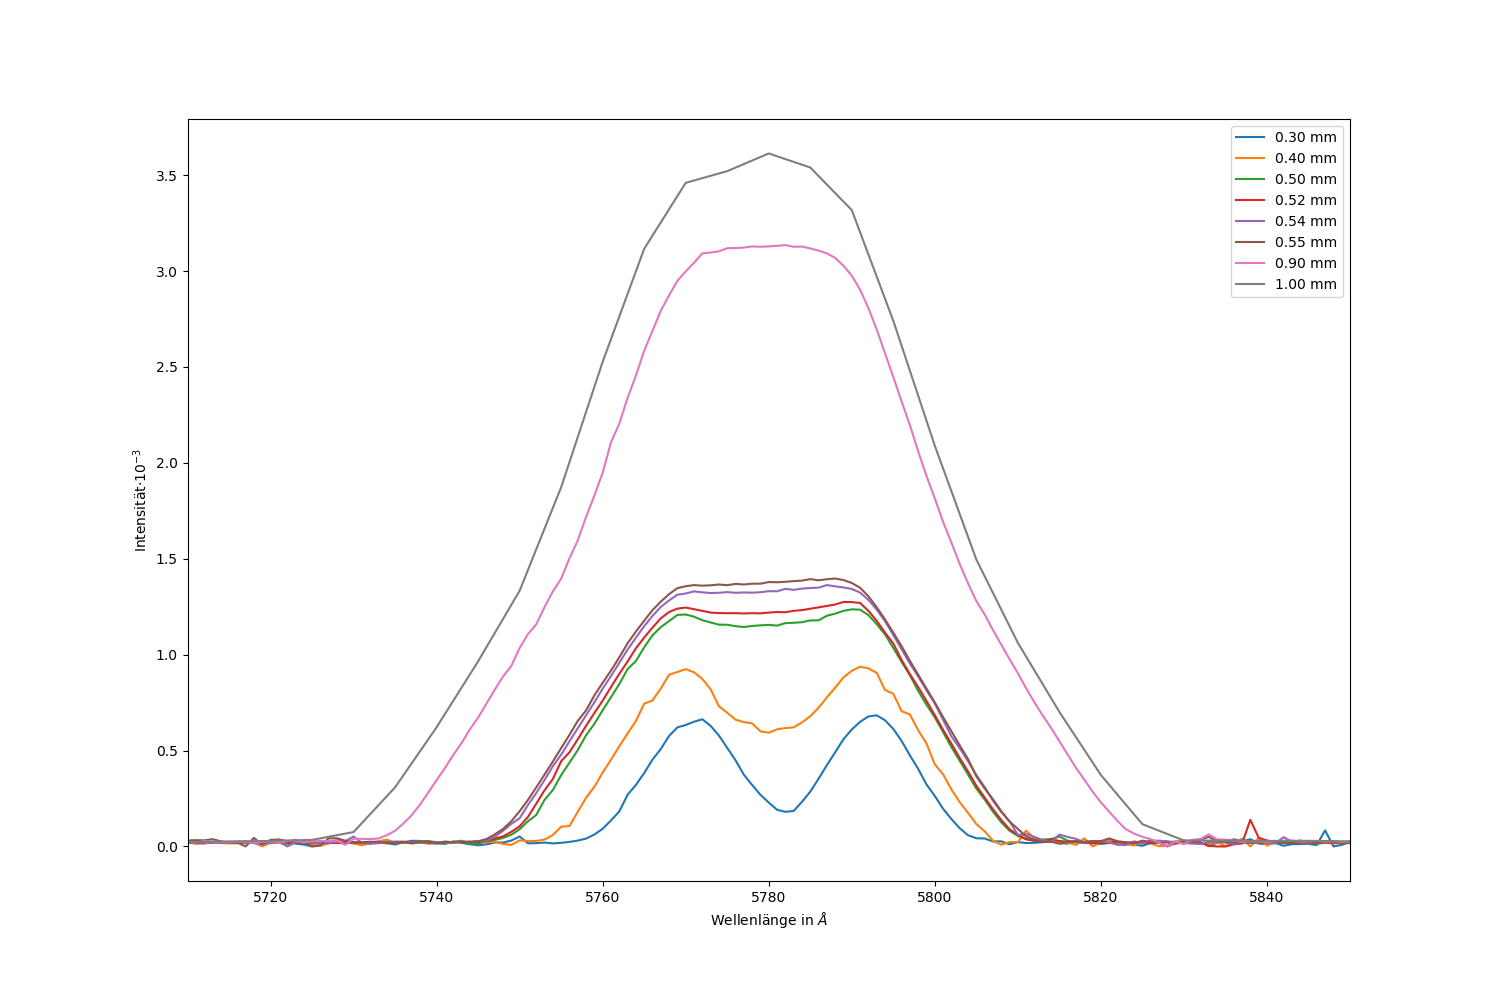
\includegraphics[width = \linewidth]{62-3-GelbeDoppellinie.png}
\end{center}
\begin{equation}
\Delta\lambda_M=\Delta\lambda_S=\sqrt{\frac{b^2}{f^2}(s_e^2+s_a^2)}
\end{equation}


Bei Annahme eines Rechteckprofils statt eines Gaußprofils und $s_e=s_a$:
\begin{equation}
\Delta\lambda_M=\sqrt{2}\frac{b}{f}\cdot s = \sqrt{2}\cdot \frac{0,5}{1200\cdot 250} =23,57nm \approx \Delta\lambda_s
\end{equation}
wobei hier wie in den Fragen zur Vorbereitung beschrieben b die Gitterkonstante und f die Brennweite des Hohlspiegels ist und der Anteil der Gitterkonstante 
vernachl\"assigbar ist (siehe FzV 5)

Die Werte f\"ur das Aufl\"oseverm\"gen der beiden Peaks, kann man aus dem Graphen lesen. Somit folgt:\\
\begin{align}
\lambda_1=577,5nm \tab \lambda_2=579,5nm\\
\Delta\lambda=2nm\\
A_{S_1}=\frac{\lambda}{\Delta\lambda_S}=432,41 \tab A_{S_2}=\frac{\lambda}{\Delta\lambda_S}=433,91\mu m
\end{align}
Die theoretische Spaltbreite berechnet sich folgenderma\ss{}en:\\
$s_{theoretisch} = \frac{\Delta\lambda f}{b}=\frac{2 \cdot 10^3 \cdot 250}{\frac{1}{1200}}= 600\mu m$\\
Beide Aufl\"osungsverm\"ogen (theoretisch und graphisch-rechnerisch) befinden sich in der gleichen Gr\"o\ss{}enordnung. Jedoch unterscheiden sie sich deutlich 
voneinander. Da man schon ab 0,55 die Peaks nicht mehr unterscheiden kann und nur noch ein Plateau ersichtlich ist, erkennt man, dass auch bei $s=600\mu m$ (wie der 
theoretische Wert) die Peaks nicht mehr zu unterscheiden sind, weshalb deutlich wird, dass der theoretische Wert nicht mit dem Experimentellen \"ubereinstimmt.
